\section{实验结果}

在实验结果的展示中,“CAT-MMT”代表本章提出的采用对比学习与对抗训练的模型,该模型没有使用\ref{sec:5_cat}小节介绍的BDTT方法。为了公平的对比各模型的结果,本节在使用了BDTT方法的模型增加“bi”后缀。可增加双向翻译训练的模型有“Transformer”、“MMT”以及“CAT-MMT”三个模型,采用了BDTT后记为“Transformer bi”、“MMT bi”以及“CAT-MMT bi”。

\subsection{翻译结果}
\label{sec:5_translation_results}
% Table generated by Excel2LaTeX from sheet 'trmmt'

\begin{table}[!htbp]
    \bicaption{在Multi30K英德翻译上的结果。}{Translation results on Multi30K EN-DE.}
    \label{tab:5_ende}
    \centering
    \footnotesize% fontsize
    \setlength{\tabcolsep}{4pt}% column separation
    \renewcommand{\arraystretch}{1.2}%row space 
    \begin{tabular}{llcccccc}
    \hline
    \multicolumn{2}{c}{\multirow{2}{*}{模型}} & \multicolumn{2}{c}{Test2016} & \multicolumn{2}{c}{Test2017} & \multicolumn{2}{c}{MSCOCO} \\\cline{3-8}
      &   & BLEU         & METEOR        & BLEU         & METEOR        & BLEU         & METEOR   \\\hline
    \multicolumn{2}{l}{~~~~SerialAtt \pcite{libovicky2018input}} & 38.7 & 57.2 & - & - & - & - \\
    \multicolumn{2}{l}{~~~~MMT-TF \pcite{yao2020multimodal}} & 39.5 & 56.9 & - & - & - & - \\
    \multicolumn{2}{l}{~~~~OVC \pcite{wang2021efficient}} & - & - & 32.4 & 52.3 & 28.6 & \textbf{48.0} \\
    \multicolumn{2}{l}{~~~~GAMMT \pcite{liu2021gumbel}} & 39.2  & 57.8  & 31.4  & 51.2  & 26.9  & 46.0  \\
    \multicolumn{2}{l}{~~~~GMMT \pcite{yin2020novel}}          & 39.8  & 57.6  & 32.2  & 51.9  & 28.7  & 47.6  \\
    \multicolumn{2}{l}{~~~~CTR-NMT}        & 39.7  & 57.5  & 32.9  & 51.7  & \textbf{29.1}  & 47.5  \\
    \multicolumn{2}{l}{~~~~CER-NMT}        & 40.2  & 57.8  & 32.5  & 52.0  & 28.3  & 47.1  \\\hline
    \multicolumn{8}{c}{本章所提方法} \\\hline
    \multicolumn{2}{l}{~~~~Transformer} & 38.5  & 57.5  & 31.0  & 51.9  & 27.5  & 47.4  \\
    \multicolumn{2}{l}{~~~~~~~~~~~~+BDTT} & 39.4  & 57.1  & 31.3  & 50.6  & 26.7  & 46.1  \\\hline
    \multicolumn{2}{l}{~~~~IGNMT} & 39.7  & 57.5  & 30.6  & 50.5  & 27.2  & 46.0  \\
    \multicolumn{2}{l}{~~~~~~~~~~~~+BDTT} & 40.0  & 57.7  & 31.6  & 51.0  & 27.7  & 46.8  \\\hline
    \multicolumn{2}{l}{~~~~CAT-NMT} & 39.8  & 57.6  & 30.6  & 50.3  & 26.6  & 45.6  \\
    \multicolumn{2}{l}{~~~~~~~~~~~~+BDTT} & \textbf{40.6}  & \textbf{58.7}  & \textbf{33.5}  & \textbf{52.6}  & 29.0  & 47.8  \\
%    CLT-MMT bi $\cup B_{\setminus X}$ & 38.5  & 57.5  & 31.0  & 51.9  & 27.5  & 47.4  \\
%    CAT-NMT bi $\cup B_{\setminus X}$ & 38.5  & 57.5  & 31.0  & 51.9  & 27.5  & 47.4  \\
     \hline
    \end{tabular}%
\end{table}%

表\ref{tab:5_ende}展示了本章提出的CAT方法在英德翻译上与其它方法的对比结果。

(1)MMT与纯文本的Transformer的实验对比中发现,增加了图片输入的MMT并没有带来全面的翻译准确率提升。在增加了BDTT方法后,两个模型的翻译准确率均有所提升。其中MMT bi与Transformer bi相比的提升更多,但两者之间的差距并不大。该部分的实验说明,简单地将图片输入给神经翻译模型很难为翻译带来有效的提升。

(2)在没有采用BDTT时,CAT-MMT的实验结果可以看到,其翻译准确率相比于MMT并没有明显的差异。CAT方法为模型带来的影响甚至没有BDTT为MMT带来的增益多。CAT方法在单独使用时似乎是无效的。

(3)采用了BDTT的CAT-MMT bi的实验中的整体表现最佳。值得注意的是,仅采用CAT时,CAT-MMT的整体表现是不如MMT的;仅采用BDTT时,MMT bi相比MMT有少许提升。如果在CAT-MMT bi中CAT没有起到额外的增益作用,那么CAT-MMT bi应该与MMT bi的结果相近。但实际结果是,当既采用CAT又采用BDTT时,CAT-MMT bi相比于MMT以及MMT bi均有着显著的提升效果。该结果说明仅采用对比对抗训练难以在小规模的数据上实现细粒度的语义表示聚类。BDTT方法通过解决目标语言与源语言之间训练不平衡的问题,使CAT能够更容易起到作用。


\begin{table}[!htbp]
    \bicaption{英日翻译与英印翻译的实验结果}{Translation results of EN-JP and EN-HI}
    \label{tab:5_enjp_enhi}
    \centering
    \footnotesize% fontsize
    \setlength{\tabcolsep}{4pt}% column separation
    \renewcommand{\arraystretch}{1.2}%row space 
    \begin{tabular}{llccc}
    \hline
    \multicolumn{2}{c}{\multirow{2}{*}{模型}} & 英日翻译~~~~ & \multicolumn{2}{c}{英印翻译}\\\cmidrule(r){3-3} \cmidrule(r){4-5}%\cline{3-5}
           &        & 测试集  & 测试集  & 挑战集~~~~  \\\hline
    
    \multicolumn{2}{l}{~~~~Transformer}    & 38.7           & 47.8           & 44.2~~~~  \\
    \multicolumn{2}{l}{~~~~~~~~~~~~+BDTT} & 38.6           & 49.4           & 45.5~~~~   \\\hline
    \multicolumn{2}{l}{~~~~IGNMT}            & 38.6           & 50.2           & 45.7~~~~  \\
    \multicolumn{2}{l}{~~~~~~~~~~~~+BDTT}        & 38.4           & 50.6           & 45.7~~~~  \\\hline
    \multicolumn{2}{l}{~~~~CAT-NMT}       & 38.8           & 50.4           & 44.8~~~~  \\
    \multicolumn{2}{l}{~~~~~~~~~~~~+BDTT}     & \textbf{39.3}  & \textbf{52.0}  & \textbf{47.0}~~~~  \\
%    CLT-MMT bi $\cup B_{\setminus X}$ & 38.5  & 57.5  & 31.0  & 51.9  & 27.5  & 47.4  \\
%    CAT-NMT bi $\cup B_{\setminus X}$ & 38.5  & 57.5  & 31.0  & 51.9  & 27.5  & 47.4  \\
     \hline
    \end{tabular}%
\end{table}%
我们同样在英日翻译和英印翻译上进行了实验。表\ref{tab:5_enjp_enhi}展示了这部分的实验结果。区别于英德翻译,在英日翻译上采用BDTT的模型并没有得到更进一步的效果,在最终的模型结果上也仅得到了0.6个BLEU值的提升。在英印翻译上的实验效果与在英德翻译上的效果是相似的。从整体上看,对比对抗训练方法在与双向翻译训练方法的配合下,能够为模型带来稳定的翻译准确率的提升。

\subsection{消融实验}
\label{sec:5_ablation_study}
\begin{table}[!htbp]
    \bicaption{消融实验结果}{Experiment results of ablation study}
    \label{tab:5_ablation_study}
    \centering
    \footnotesize% fontsize
    \setlength{\tabcolsep}{4pt}% column separation
    \renewcommand{\arraystretch}{1.2}%row space 
    \begin{tabular}{cccccccccccccc}
    %\toprule[1pt]
    \hline
    \multicolumn{2}{c}{\multirow{2}*{模型}} & \multicolumn{6}{c}{英德翻译} &\multicolumn{2}{c}{英日翻译~~~~} & \multicolumn{4}{c}{英印翻译}\\\cmidrule(r){3-8} \cmidrule(r){9-10} \cmidrule(r){11-14}%\cline{3-8}
      &   & \multicolumn{2}{c}{Test2016}& \multicolumn{2}{c}{Test2017}& \multicolumn{2}{c}{MSCOCO}& \multicolumn{2}{c}{测试集} & \multicolumn{2}{c}{测试集} & \multicolumn{2}{c}{挑战集}  \\\hline
    
    \multicolumn{2}{l}{CAT-NMT~+~BDTT}   & \textbf{40.6}  &  & \textbf{33.5}  &  & \textbf{29.0}  &   & \textbf{39.3}  &  & \textbf{52.0}  &   & \textbf{47.0}  \\
    & \qquad -w/o $B_{\setminus X}$  & 40.0  & (-0.6)  & 31.0  & (-2.5)  & 27.4  & (-1.6)  & 38.7  & (-0.6)  & 50.7  & (-1.3)  & 44.5  & (-2.5)   \\
    & \qquad -w/o $N_{AS}$           & 39.9  & (-0.7)  & 32.0  & (-1.5)  & 27.8  & (-1.2)  & 39.0  & (-0.3)  & 51.2  & (-0.8)  & 45.6  & (-1.4)    \\\hline
    \multicolumn{2}{l}{CAT-NMT}      & 39.8  &         & 30.6  &        & 26.6  &         & 38.8  &         & 50.4  &         & 44.8  & \\
    & \qquad -w/o $B_{\setminus X}$  & 39.6  & (-0.2)  & 30.6  & (0.0)  & 27.0  & (+0.4)  & 38.4  & (-0.4)  & 50.5  & (+0.1)  & 44.5  & (-0.3) \\
    & \qquad -w/o $N_{AS}$           & 39.8  & (0.0)   & 30.9  & (+0.3) & 26.5  & (-0.1)  & 38.5  & (-0.3)  & 50.4  & (0.0)   & 44.6  & (-0.2)  \\
%    CLT-MMT bi $\cup B_{\setminus X}$ & 38.5  & 57.5  & 31.0  & 51.9  & 27.5  & 47.4  \\
%    CAT-NMT bi $\cup B_{\setminus X}$ & 38.5  & 57.5  & 31.0  & 51.9  & 27.5  & 47.4  \\

    
     \hline
    \end{tabular}%
\end{table}%
为了分析本章为对比对抗训练所设计的负样本在模型中是否起到了作用,本节将针对CAT-MMT和CAT-MMT bi设置消融实验。

实验结果如表\ref{tab:5_ablation_study}所示,其中“w/o $B_{\\X}$”代表同批数据下的其它样本从负样本集$N$中移除。该条件下,负样本集$N$的大小为$|N|=|N_{AS}|=2$。“w/o $N_{AS}$”代表将对抗样本从负样本集$N$中移除。没有了$N_{AS}$,CAT方法将退化为一般的对比学习方法,不再进行细粒度的语义聚类。

从表\ref{tab:5_ablation_study}中的结果可以看到,移除$B_{\\X}$或$N_{AS}$的实验设置对CAT-MMT bi有着较大的影响,对CAT-MMT的影响则可以忽略不计。消融后的模型表现与表\ref{tab:5_ende}和表\ref{tab:5_enjp_enhi}中MMT和MMT bi相似,即与一般的直接输入图片信息的神经翻译模型相似。从该实验结果中可以得到以下两个结论:

(1)$B_{\\X}$是对比学习有效的一个先决条件,仅采用对抗样本集$N_{AS}$作负样本集,即使CAT方法与BDTT配合也无法达到理想的效果。在$B_{\\X}$的帮助下,模型可以在语义空间中进行细粒度的语义聚类。从而将互为翻译的句子聚类到一起,将不同语义的句子分开。然而仅采用$B_{\\X}$的情况下模型的翻译准确率依旧不理想,这说明翻译模型还没有对视觉信息敏感。

(2)$N_{AS}$是对比对抗训练有效的原因。增加了对抗样本作为负样本后,模型需要进行更细粒度的语义聚类才能把对抗样本与正样本区分开。如果模型能够成功地区分$X+\tilde{I}$与$X+I$,那么就必须从图片中获得差异化的信息。而根据本章对解码模块以及对比学习模块的设计可知,对比学习模块能够感知到图片信息的唯一途径就是将其融合到文本的表示中。只有当图片中包含了与文本内容相近的语义信息时,才能将其作为正样本使其与译文的语义靠近。

综合以上实验结果与分析,当负样本集同时包含$B_{\\X}$或$N_{AS}$时,在双向翻译训练的配合下对比对抗训练方法能够为融合图片信息的神经机器翻译模型带来有效的翻译准确率的提升。
%该实验结果说为负样本集增加对抗样本集$B_{\\X}$是有效的。在$B_{\\X}$的帮助下,对比损失能够在更细粒度的语义空间中进行语义的聚类,从而使模型将输入的图片信息融合到文本的表示中。

\subsection{双向翻译训练分析}
\label{sec:5_bdtt_analysis}

在前面小节的实验结果中,双向翻译训练方法为模型的翻译质量提升起到了关键的作用。因此,有必要针对BDTT实施进一步地分析,从而展示其真正的作用。为此,我们记录了CAT-MMT bi和CAT-MMT在训练过程中输入样本之间的余弦距离的变化情况。该实验在Multi30K的验证集上每2000步进行一次记录。在\ref{sec:5_cat}小节和\ref{sec:5_translation_results}小节中我们解释到,BDTT是通过优化编码器对目标语言句子$Y$的表示能力使CAT方法有效。因此,本小节将以$X+I$为基线,记录$X$、$Y$以及$X+\tilde{I}$这三者与$X+I$之间在训练过程中的余弦距离变化。

\begin{figure}[!htbp]
    \centering
    \begin{subfigure}[b]{0.5\textwidth}
      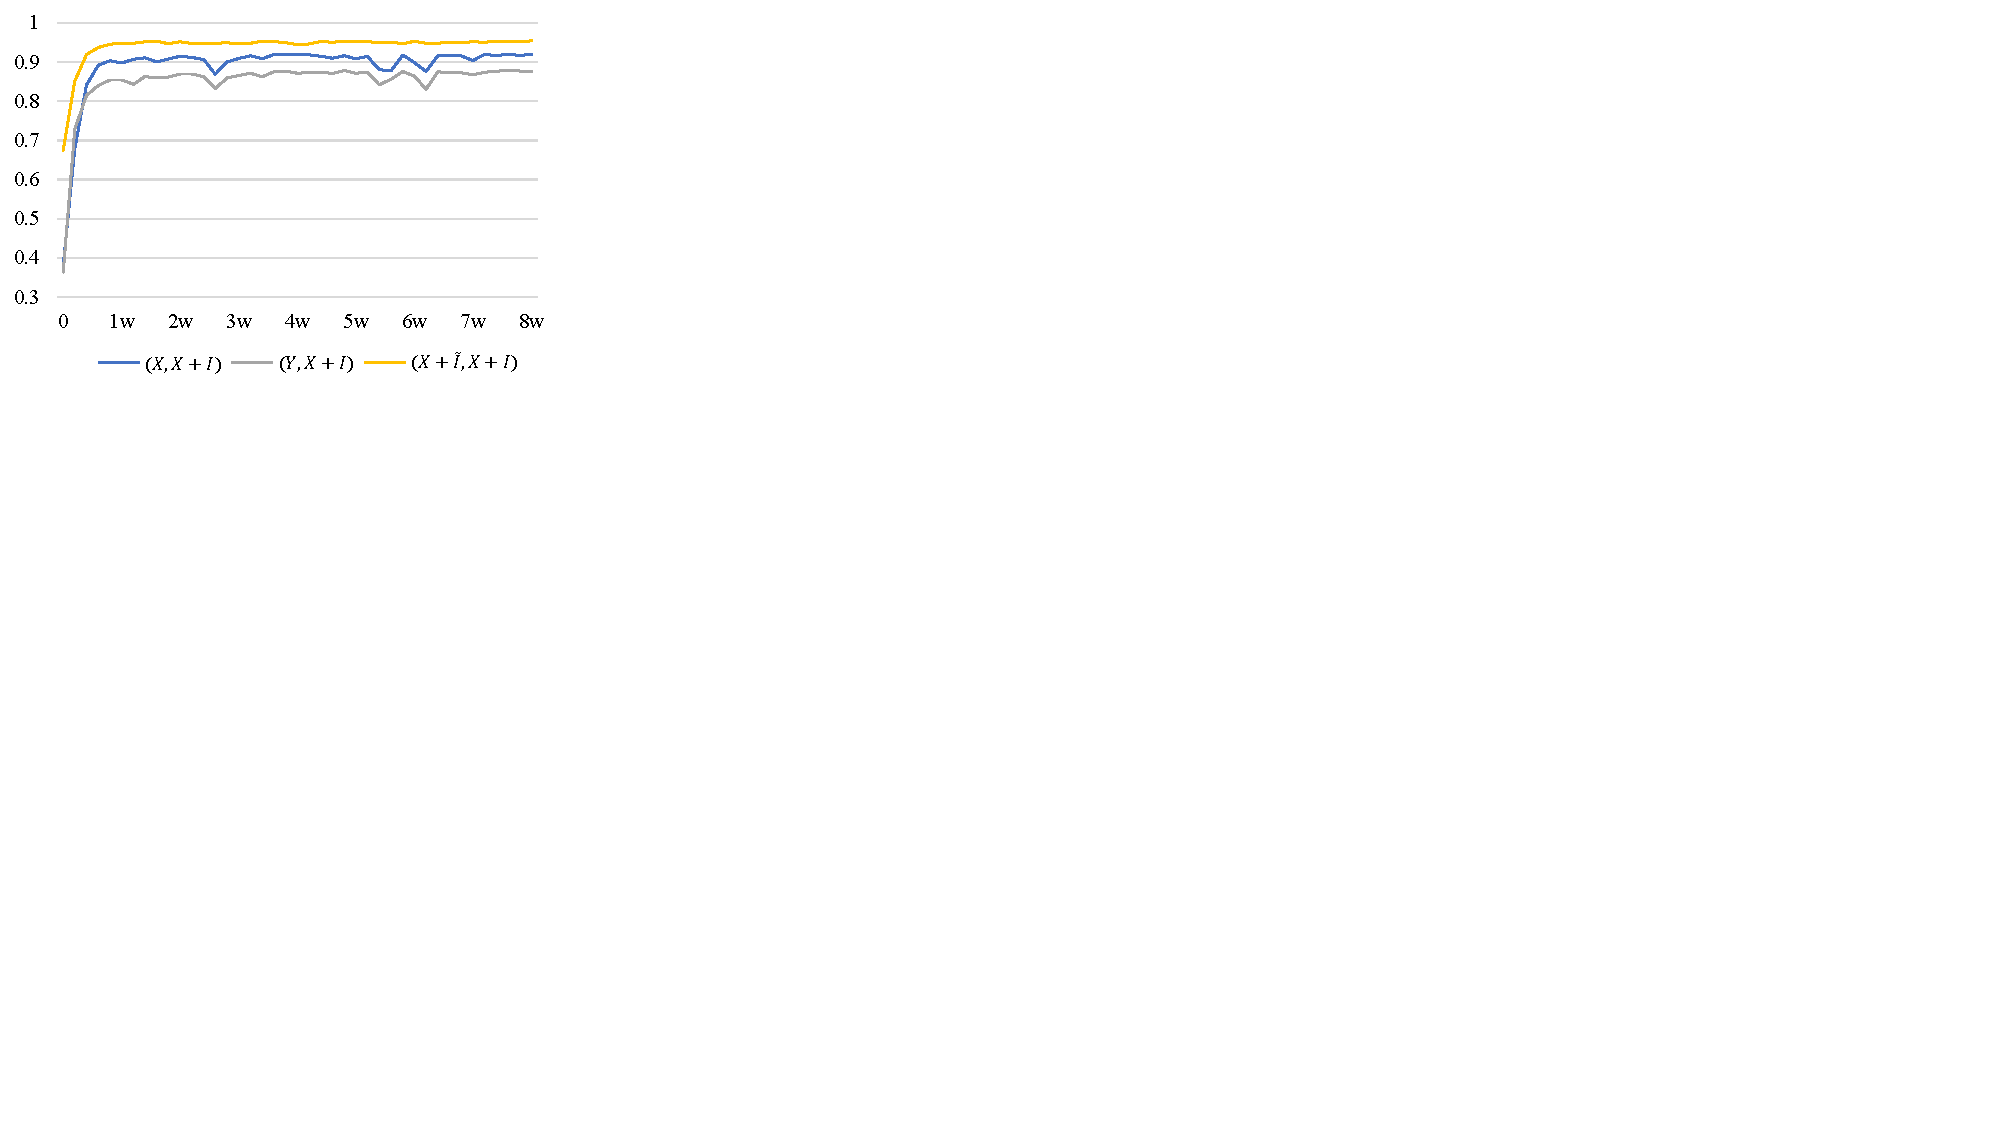
\includegraphics[width=\textwidth]{Img/fig_5_training_cat_mmt_bi.pdf}
      \caption{CAT-NMT~+~BDTT}
      \label{fig:5_training_cat_mmt_bi}
    \end{subfigure}%
    ~% add desired spacing
    \begin{subfigure}[b]{0.5\textwidth}
      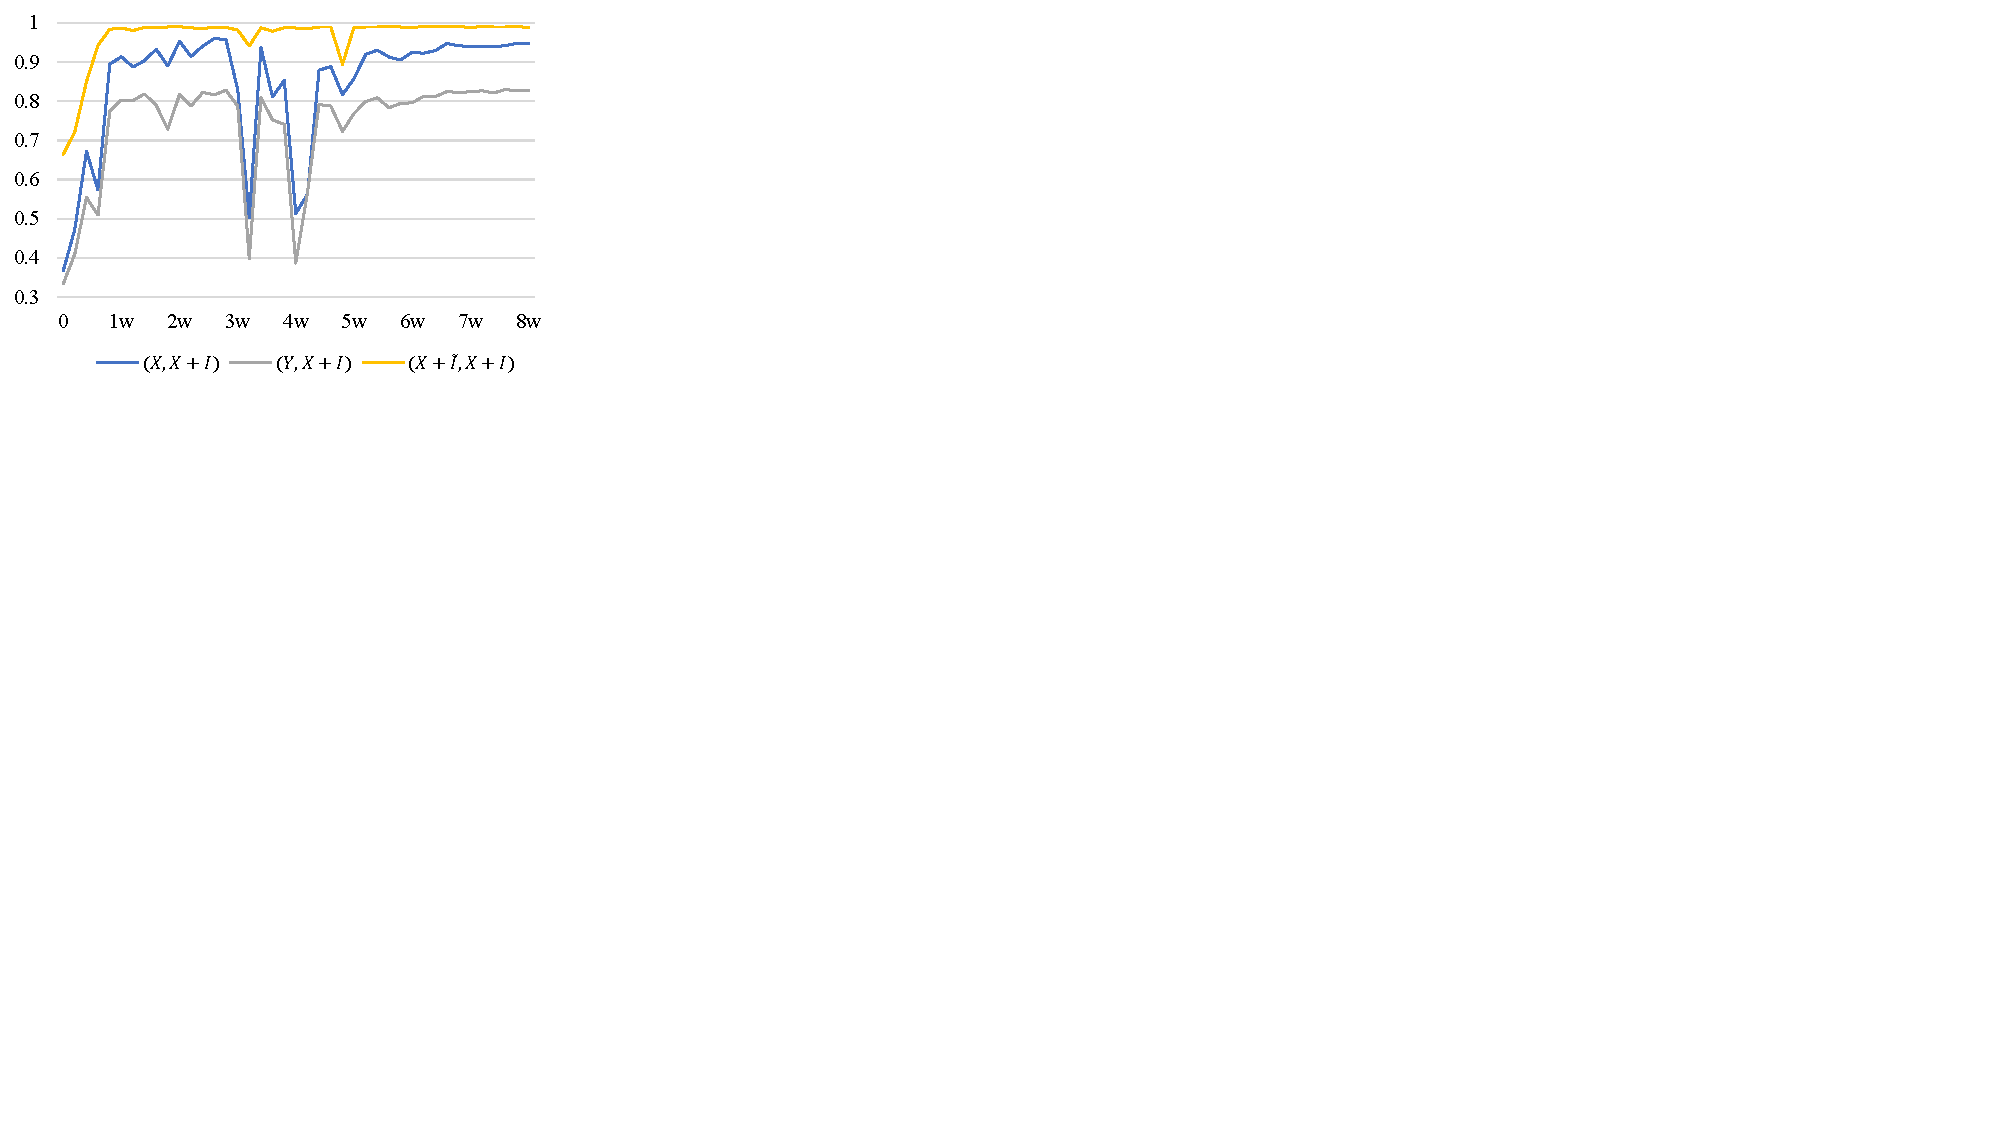
\includegraphics[width=\textwidth]{Img/fig_5_training_cat_mmt.pdf}
      \caption{CAT-NMT}
      \label{fig:5_training_cat_mmt}
    \end{subfigure}
    \bicaption{双向翻译训练方法在模型训练过程中对样本余弦距离的影响}{Influence of BDTT on cosine distance among samples during model training}
    \label{fig:5_training}
\end{figure}

实验结果如图\ref{fig:5_training}所示,其中$X+I$与$Y$之间的余弦距离在没有BDTT的情况下的收敛过程产生了急剧的波动。这表明BDTT方法确实能够帮助目标语言得到好的编码表示。在仅使用CAT方法的情况下,对比损失很难针对目标语言从开始训练一个好的表示向量。除以上观察外,该实验结果还可以得到以下结论:

(1)尽管在BDTT的配合下对比损失能够起到很好的作用,但$X+I$与$X+\tilde{I}$之间的余弦距离依旧很近(接近1.0)。这表明Multi30K验证集中的大部分句子并不需要视觉信息的帮助。这与我们的假设是一致的。

(2)图\ref{fig:5_training_cat_mmt_bi}各样本之间的余弦相似度很快就收敛到了一个稳定的范围内。这说明在BDTT的帮助下,对比损失函数更像是对源语言和目标语言表示空间的限制。使得在进行翻译优化的过程中,保持住样本之间的相对距离。

(3)$X$与$X+I$之间的余弦距离大于$X+\tilde{I}$与$X+I$之间的余弦距离。然而,$X$中并没有携带错误的图片信息,该结果实际上与预期相悖。一个可能的原因是,模型越多地关注“图片模态”中的信息,因为没有输入图片而导致的神经元连接的丢失所带来的负面影响就越大。这一点我们将在后面的小节中进一步证明。

(4)尽管相对距离最远的是目标语言$Y$,这样的结果也是可以理解的。在将目标端或源端句子的隐层单元传递给对比学习模块前,我们仅对隐层向量做了平均池化。在没有任何映射的情况下,将不同语言句子的平均表示向量映射到一个极度集中的区域内实际上是不太可能的。

\subsection{对抗评估}
\label{sec:5_adversarial_evaluation}
\begin{table}[htbp]
    \bicaption{对抗评估实验结果}{Experiment results of adversarial evaluation}
    \label{tab:5_adversarial_evaluation}
    \centering
    \footnotesize% fontsize
    \setlength{\tabcolsep}{3pt}% column separation
    \renewcommand{\arraystretch}{1.0}%row space 
    \begin{tabular}{lccccccccccccc}
    \hline
    \multicolumn{2}{c}{\multirow{2}*{模型}} & \multicolumn{6}{c}{英德翻译} & \multicolumn{2}{c}{英日翻译~~~~} & \multicolumn{4}{c}{英印翻译}\\\cmidrule(r){3-8} \cmidrule(r){9-10} \cmidrule(r){11-14}%\cline{3-8}
      &   & \multicolumn{2}{c}{Test2016}& \multicolumn{2}{c}{Test2017}& \multicolumn{2}{c}{MSCOCO}& \multicolumn{2}{c}{测试集} & \multicolumn{2}{c}{测试集} & \multicolumn{2}{c}{挑战集}  \\\hline
    
    CAT-NMT BDTT & $X+I$  & 40.6 &        & 33.5 &       & 29.0 &       & 39.3 &       & 52.0 &        & 47.0 & \\
    & $X$               & 40.3 &(-0.3)  & 32.1 &(-1.4) & 27.1 &(-1.9) & 38.7 &(-0.6) & 41.8 &(-10.2) & 35.5 &(-11.5) \\
    & $X+\tilde{I}$     & 40.4 &(-0.2)  & 31.6 &(-1.9) & 27.1 &(-1.9) & 38.9 &(-0.4) & 49.3 &(-2.7)  & 43.4 &(-3.6)  \\\hline
    IGNMT BDTT & $X+I$      & 40.0 &        & 31.6 &       & 27.7 &       & 38.4 &       & 50.6 &        & 45.7 & \\
    & $X$               & 39.6 &(-0.4)  & 30.8 &(-0.8) & 27.2 &(-0.5) & 38.2 &(-0.2) & 49.1 &(-1.5)  & 39.8 &(-5.9)  \\
    & $X+\tilde{I}$     & 39.9 &(-0.1)  & 31.6 &(0.0)  & 27.7 &(0.0)  & 38.5 &(+0.1) & 50.3 &(-0.3)  & 45.3 &(-0.4)  \\\hline
    
    CAT-NMT & $X+I$     & 39.8 &        & 30.6 &       & 26.6 &       & 38.8 &        & 50.4 &        & 44.8 & \\
    & $X$               & 38.9 &(-0.9)  & 30.3 &(-0.3) & 25.9 &(-0.7) & 38.7 &(-0.6)  & 48.6 &(-1.8)  & 35.8 &(-9.0) \\
    & $X+\tilde{I}$     & 39.4 &(-0.4)  & 30.5 &(-0.1) & 26.0 &(-0.6) & 38.9 &(-0.4)  & 50.0 &(-0.4)  & 44.1 &(-0.7)  \\\hline
    IGNMT & $X+I$         & 39.7 &        & 30.6 &       & 27.2 &       & 38.6 &        & 50.2 &        & 45.7 & \\
    & $X$               & 39.4 &(-0.3)  & 30.1 &(-0.5) & 26.7 &(-0.5) & 38.2 &(-0.2)  & 50.4 &(+0.2)  & 43.2 &(-2.5)  \\
    & $X+\tilde{I}$     & 39.6 &(-0.1)  & 30.5 &(-0.1) & 27.3 &(+0.1) & 38.5 &(+0.1)  & 50.1 &(-0.1)  & 45.7 &(-0.0)  \\
%    CLT-MMT bi $\cup B_{\setminus X}$ & 38.5  & 57.5  & 31.0  & 51.9  & 27.5  & 47.4  \\
%    CAT-NMT bi $\cup B_{\setminus X}$ & 38.5  & 57.5  & 31.0  & 51.9  & 27.5  & 47.4  \\

     \hline
    \end{tabular}%
\end{table}%
图片辅助式的神经机器翻译普遍存在着对视觉信息不敏感的问题,所以使用对抗样本来评估模型对视觉信息的敏感度成为每种方法必须经过的测试。本节将针对本章所提出的方法通过改变输入的图片来测试模型对视觉信息的敏感度。其中“$X+I$”代表着为模型输入与原文对应的图片,“$X+\tilde{I}$”代表输入与原文不一致的图片,“$X$”代表只输入原文不输入图片。如表\ref{tab:5_adversarial_evaluation}所示为实验结果,从该实验结果中可以得到以下信息:

(1)对抗评估对CAT-MMT bi带来的影响最大。这表明在BDTT的帮助下,CAT-MMT bi能够从图片中获取信息从而带来翻译质量的提升。对抗评估对CAT-MMT的影响也有,但相对更小。从CAT-MMT在$X+\tilde{I}$和$X$两种输入下的结果中看,模型似乎只是对是否有视觉信息感兴趣,但对视觉信息中的内容并不感兴趣。

(2)相比于$X+\tilde{I}$,$X$对翻译准确率的负面影响更大。这一方面说明与原文不一致的图片作为一种噪声输入对模型是有一定正面的影响,例如提升模型的鲁棒性或做为一种正则方法提升了模型的翻译质量\pcite{wu2021good}。另一个原因是,当模型对输入图片中的视觉信息越敏感,模型在编码的过程中就越会去“注意”“视觉模态”带来的信息。当输入为纯文本时,编码过程将丧失对“视觉模态”的神经元连接,在一定程度上造成了对纯文本输入不兼容的问题。因此带来的负面影响更严重。

(3)英德翻译的Ambiguous MSCOCO 2017和英印翻译的挑战集都是为歧义词问题而设计的。相比于其它的测试集,针对歧义词的测试集受对抗输入的影响更大。但对Ambiguous MSCOCO 2017的影响明显小于对英印翻译的挑战集,这说明尽管是针对歧义词而设计,但Ambiguous MSCOCO 2017内部的歧义词问题并不严重。

(4)英印翻译的HVG数据集受到对抗样本的影响最大。这是因为HVG数据集中对图片的描述更简单也更短,使得模型更容易做到跨模态的信息融合。然而,该结果同样表明了模型对视觉信息越敏感,模型的鲁棒性也就越差。面对对抗样本的攻击时,输出错误结果的概率就越大。

(5)尽管对抗样本降低了模型的翻译准确率,但是CAT-MMT bi的结果依然超过了表\ref{tab:5_ende}和表\ref{tab:5_enjp_enhi}中纯文本模型的结果。这同样说明了噪音输入具有通过为模型提升鲁棒性来提升翻译准确率的能力。这与\tcite{elliott2018adversarial,wu2021good,li2021vision}中有着相似的结论。


\subsection{样例分析}
图\ref{fig:5_case_ende}、图\ref{fig:5_case_enjp}和图\ref{fig:5_case_enhi}分别展示了CAT-MMT bi模型在三个不同的数据集上的翻译案例。我们选择了带有歧义词的句子,歧义词包含“passing”、“reached”以及“stamp”。为了方便比较,我们将模型的结果通过Google翻译系统\footnote{https://translate.google.com}翻译到了英文,并在每个句子下面展示。该实验结果表明了图片信息能够在很大程度上影响歧义词的翻译。在图\ref{fig:5_case_ende}英德翻译和图\ref{fig:5_case_enhi}英印翻译在$X+\tilde{I}$作为输入情况下出现了漏翻的问题。说明错误的图片信息影响到了歧义词的翻译过程。当纯文本$X$作为模型输入时,几乎所有的翻译结果都是错的,并与原来的词义相差甚远。这验证了我们之前的想法,说明模型越依赖视觉信息,其鲁棒性反而越差。

\begin{figure}[!htbp]
    \centering
    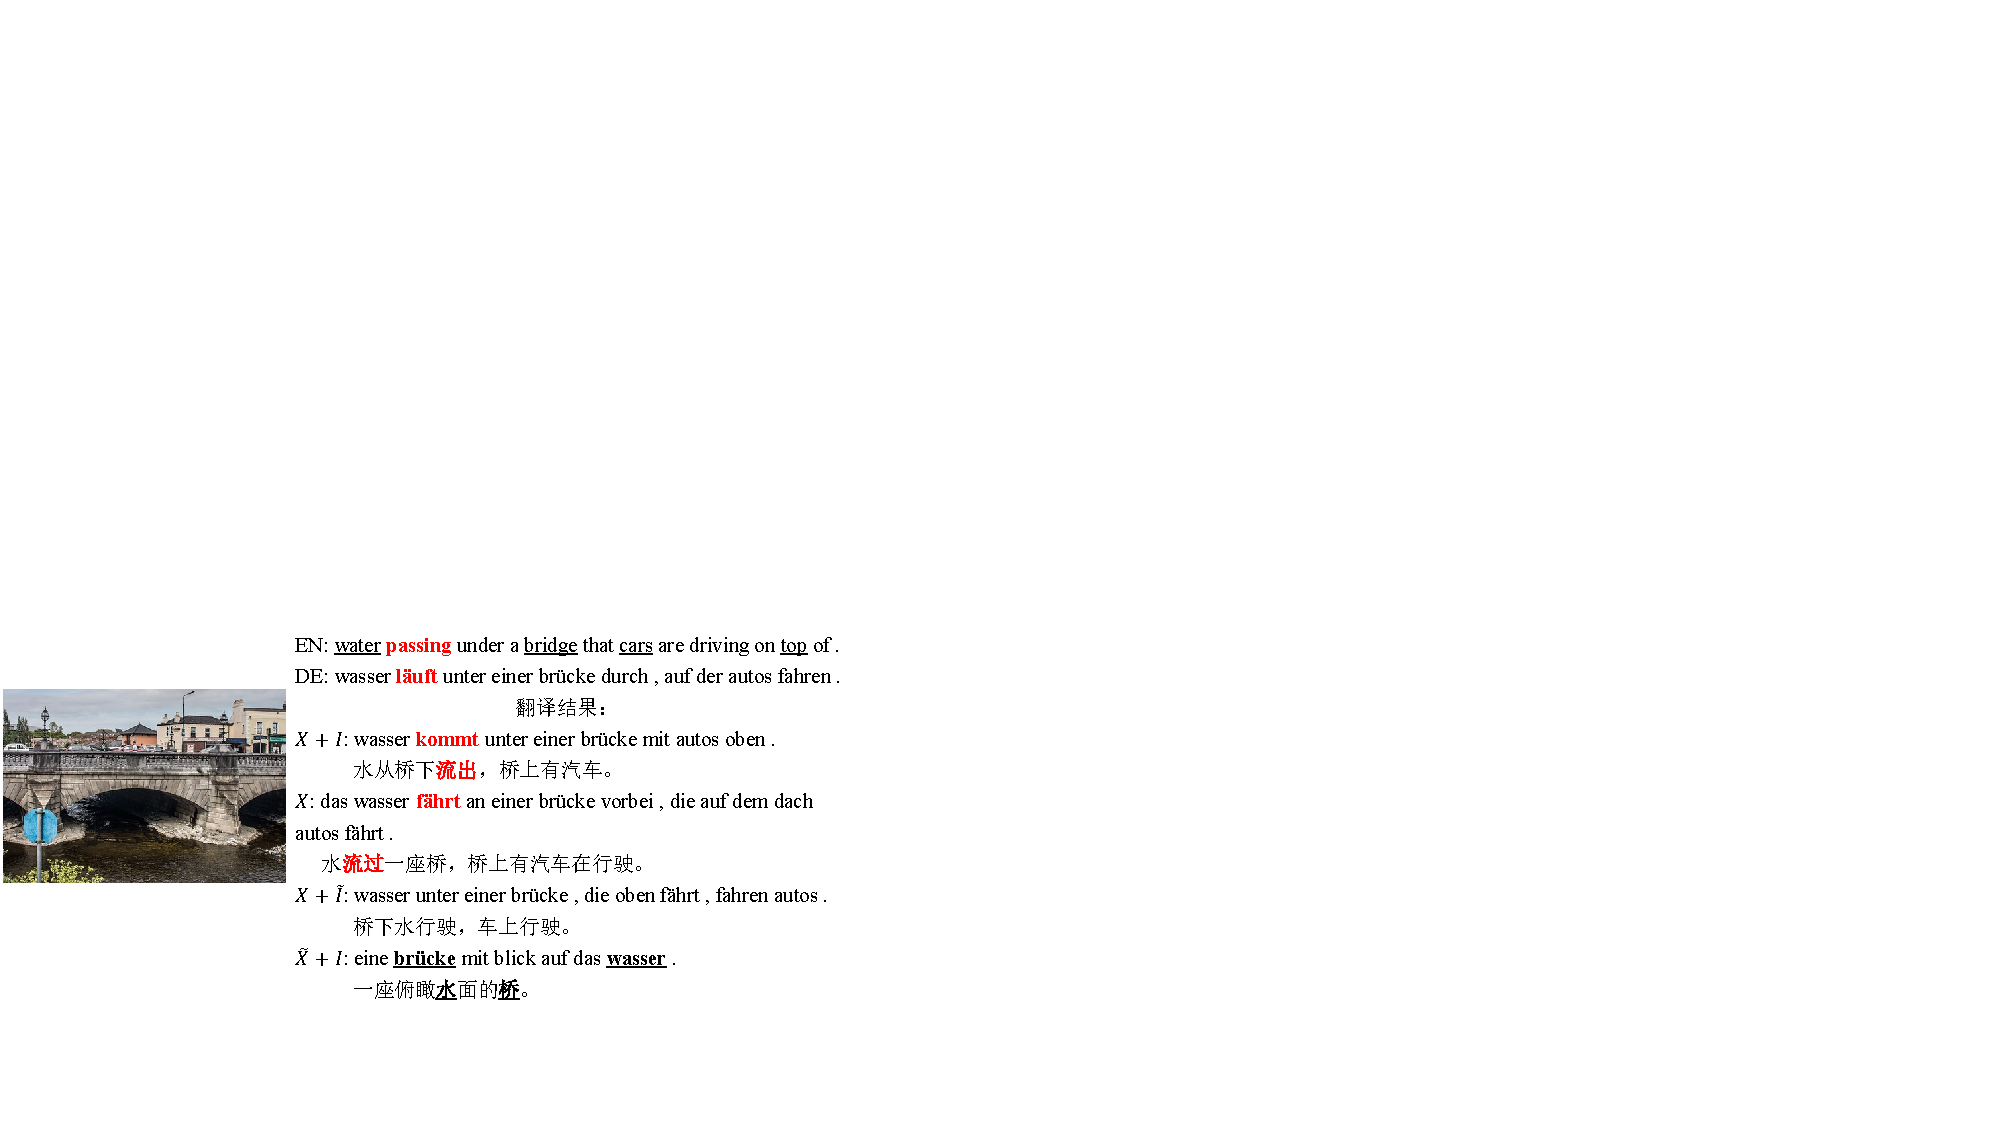
\includegraphics[scale=1.0]{Img/fig_5_case_ende.pdf}
    \bicaption{英德翻译案例}{Translation case for EN-DE}
    \label{fig:5_case_ende}
\end{figure}
\begin{figure}[!htbp]
    \centering
    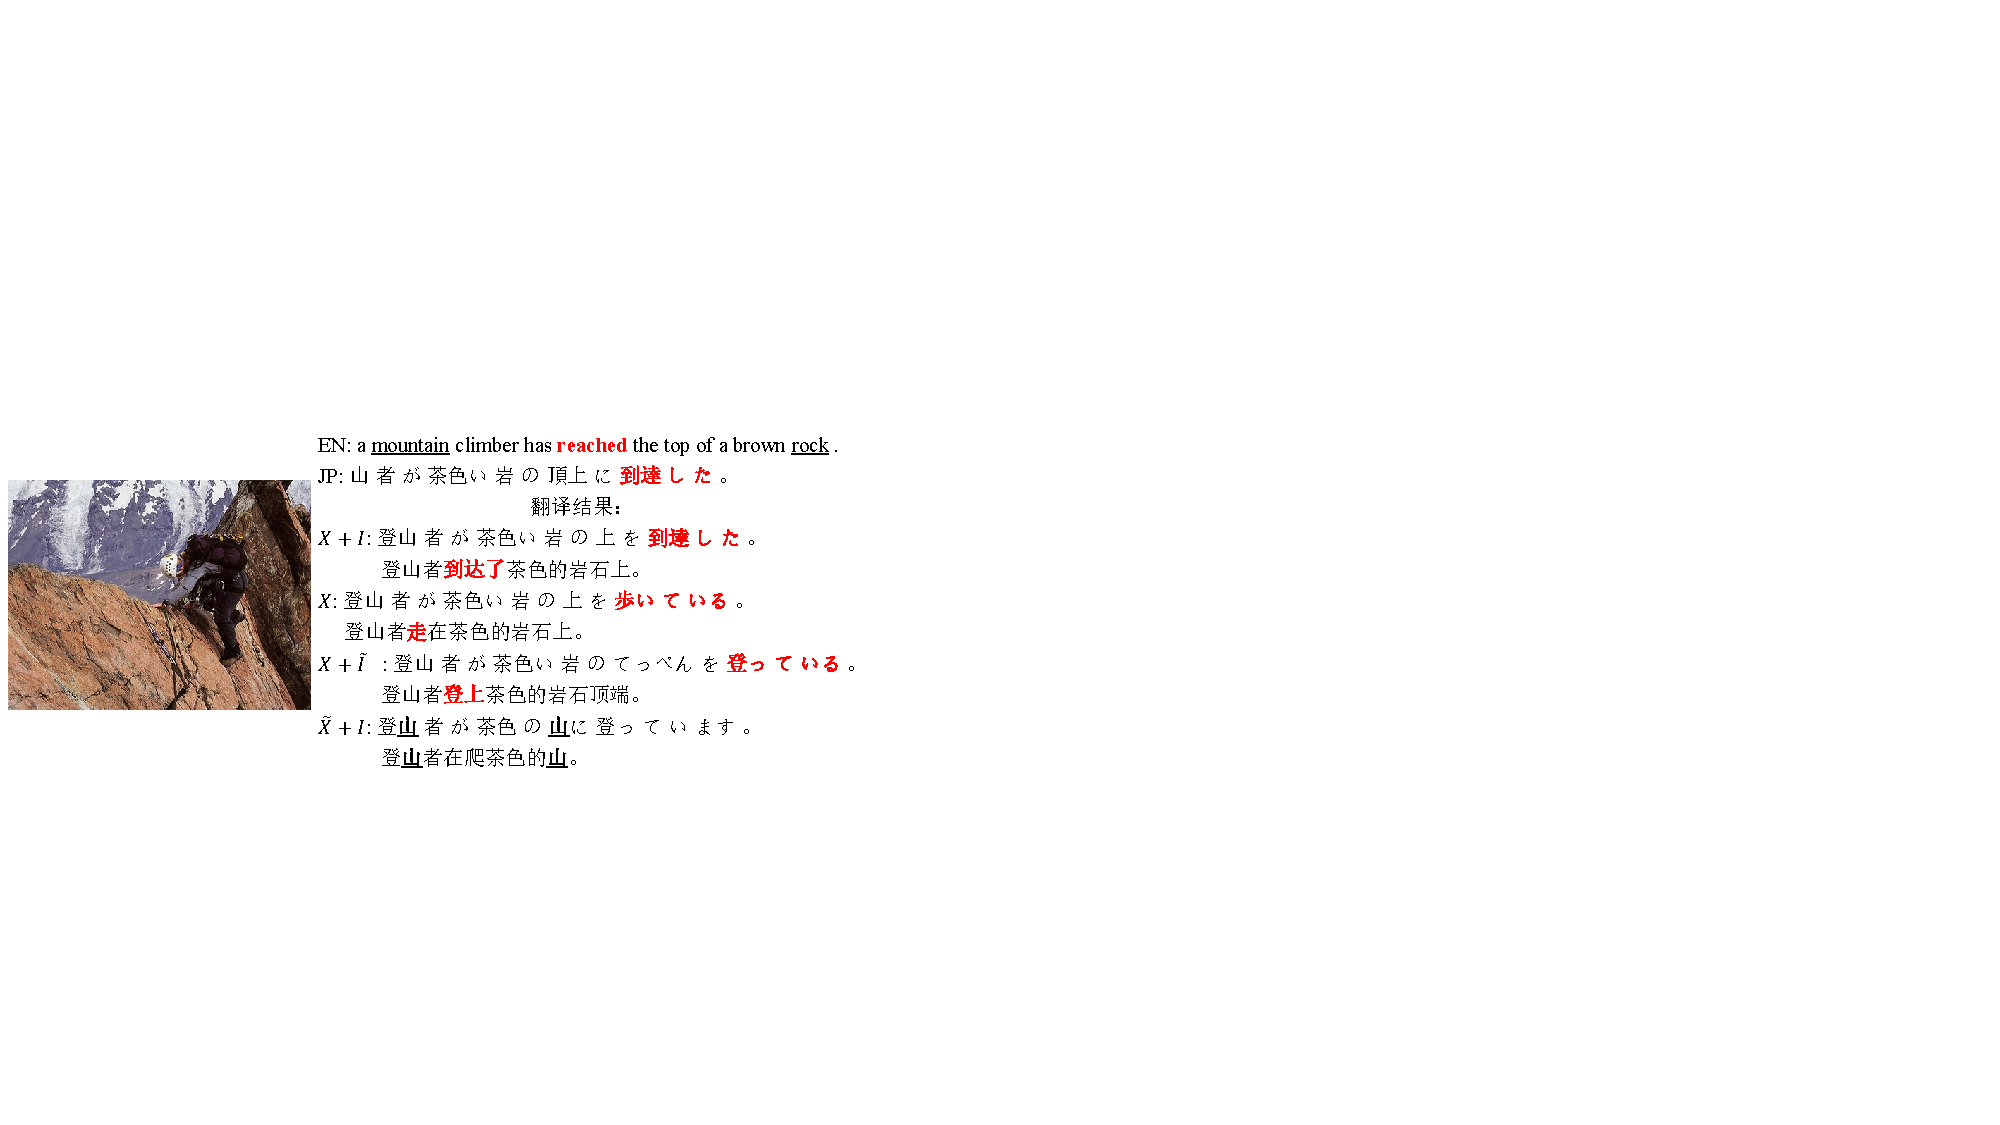
\includegraphics[scale=1.0]{Img/fig_5_case_enjp.pdf}
    \bicaption{英日翻译案例}{Translation case for EN-JP}
    \label{fig:5_case_enjp}
\end{figure}
\begin{figure}[!htbp]
    \centering
    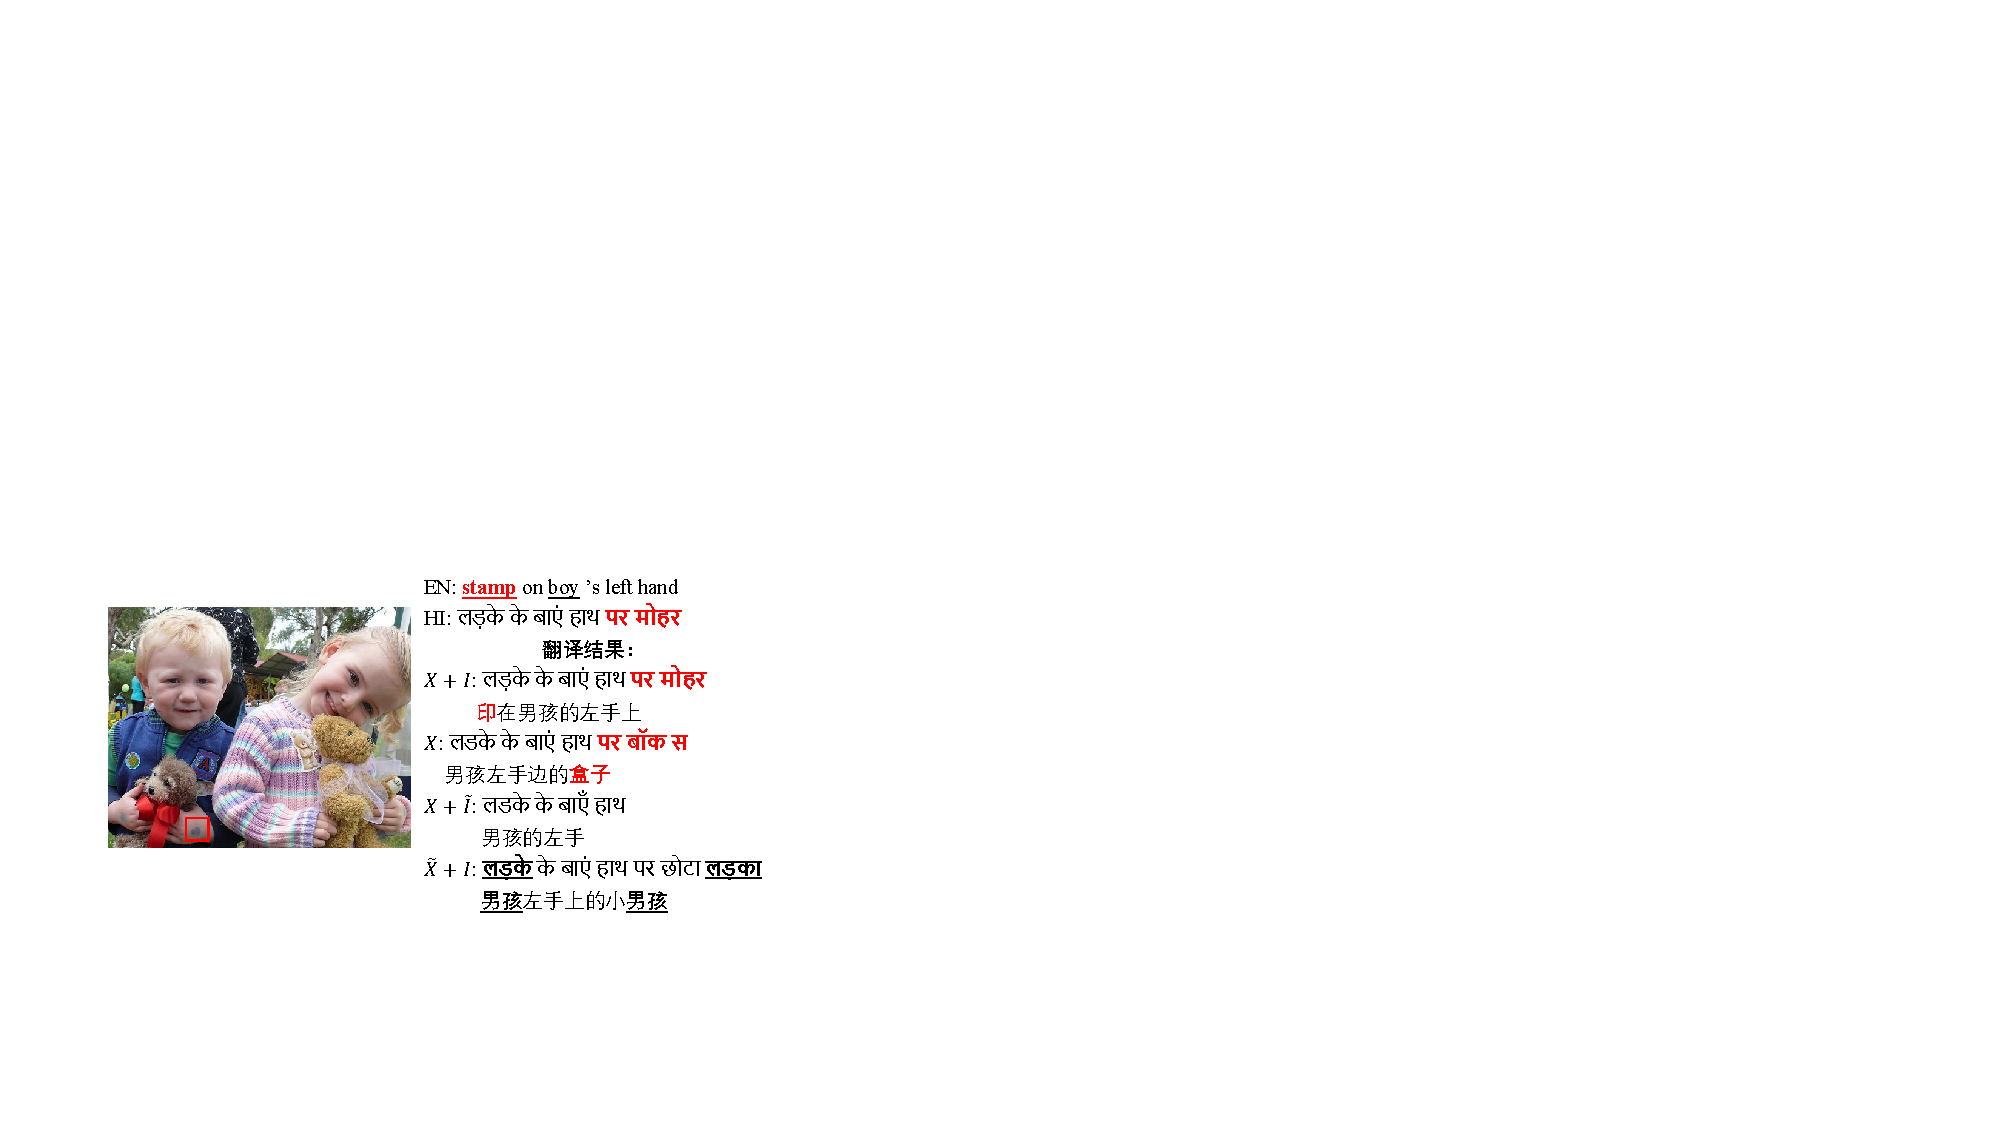
\includegraphics[scale=1.0]{Img/fig_5_case_enhi.pdf}
    \bicaption{英印翻译案例}{Translation case for EN-HI}
    \label{fig:5_case_enhi}
\end{figure}
我们同样测试了模型在输入退化文本情况下通过图片补全信息的能力。文本的退化方案与\ref{sec:5_cat}小节中介绍的针对对抗样本$\tilde{X}+\tilde{I}$的方法相同,即将句子中与视觉目标相对应的名词替换为“<mask>”。图图\ref{fig:5_case_ende}、图\ref{fig:5_case_enjp}和图\ref{fig:5_case_enhi}中所有源语言中带有下划线的词为选作退化的词。在$\tilde{X}+I$的翻译结果中重构出的对应词也同样带有下划线。图\ref{fig:5_case_ende}的结果展示出,在图中有明显目标的“water”和“bridge”成功地在翻译中被还原。然而,整体的翻译结果却非常差。这是因为这个句子中有太多的词被掩码替换,破坏了整个句子的语义完整性,仅依靠图片很难补全完整的语义信息。图\ref{fig:5_case_enjp}中,为了降低难度,我们只选择了两个词“mountain”和“rock”。结果中“mountain”成功地还原了出来。但是根据源语言的句子,其还原出来的位置是错的。图\ref{fig:5_case_enhi}展示了一个简单的句子,“boy”成功地得到了还原,“stamp”则没有。

上述结果证明了我们的方法将视觉信息融合到文本表示中的能力。当文本中出现歧义词时,模型可以准确翻译这些歧义词。替换或删除输入图像会极大地影响翻译结果。
上述分析还展示了我们的模型从匹配图像中还原退化句子缺失的信息的能力。模型可以从图像中捕获部分信息。实验结果还表明编码过程是文本主导的过程,输入文本的完整性在很大程度上影响翻译结果,图片信息只能起到辅助的作用。